\chapter{Estudos de caso}
\label{SectionEstudosDeCaso}
Neste capítulo, será estudado uma rede elementar de 4 barras e 4 linhas de transmissão (na seção \ref{SectionRedePequena}). A rede elementar tem um papel fundamental para compreensão de todos os passos do método, além de servir como calibração e teste para todas as modificações subsequentes. Para cada modificação no código de referência, ainda que pequena, deve ser retestado tendo a saída desta rede como parâmetro.
\section{Rede de 4 barras e 4 linhas de transmissão}
\label{SectionRedePequena}
Considere a rede de quatro barras e quatro linhas de transmissão na figura \ref{FigRede4barrasLinearizado}.\\
\begin{figure}[!htb]
\caption{Rede de quatro barras e quatro linhas de transmissão}
 \centering % para centralizarmos a figura
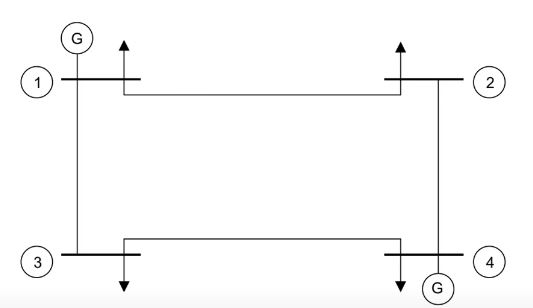
\includegraphics[width=8cm]{figuras/Linearizado4barrasValida.JPG}
\label{FigRede4barrasLinearizado}
\end{figure}

\subsection{Dados do Problema}
Tem-se $S_{base}=100MVA$.\\ 
Na tabela \ref{t_redePequenaBarras} estão os dados das barras do problema apresentado na seção \ref{SectionRedePequena}.\\
\begin{table}[!htb]
\centering
\caption{Barras da rede de quatro barras}
\begin{tabular}{lllllll}
\hline
Barra & V (pu) & $\theta$ (graus) & Pg (MW) & Qg (MVar) & Pc (MW) & Qc (MVar)   \\ \hline
1 & 1,00 & 0 & - & - & 50 & 30,99   \\
2 & - & -& 0& 0 & 170 & 105,35    \\
3 & - & - & 0 & 0 & 200 & 123,94   \\
4 & 1,02  & - & 318 & - & 80 & 49,58 \\ \hline
\end{tabular}
\label{t_redePequenaBarras}
\end{table}

Na tabela \ref{t_redePequenaRamos} estão os dados das impedâncias séries dos ramos do problema apresentado na seção \ref{SectionRedePequena}.
\begin{table}[!htb]
\centering
\caption{Barras da rede de quatro barras}
\begin{tabular}{lll}
\hline
Ramos & r (pu) & x (pu) \\ \hline
1-2 & 0.01008 & 0.05040 \\
1-3 & 0.00744 & 0.03720 \\
2-4 & 0.00744 & 0.03720 \\
3-4 & 0.01272 & 0.06360 \\ \hline
\end{tabular}
\label{t_redePequenaRamos}
\end{table}
\subsection{Equacionamento matriz P}
A matriz $P$ será calculada a partir da tabela \ref{t_redePequenaBarras} e será uma matriz da potência gerada menos a potência consumida, como mostrado em \ref{RedePequenaP}. 
\begin{equation}
    P = \left[ 
    \begin{matrix} 
        0 - 1,70 \\
        0 - 2,00 \\
        3,18 - 0,80
    \end{matrix} \right]=\left[ 
    \begin{matrix} 
        -1,70 \\
        - 2,00 \\
        2,38
    \end{matrix} \right]   
    \label{RedePequenaP}
\end{equation}

\subsection{Equacionamento matriz B'}
A matriz $B'$ apresentada na equação \ref{redePequena_Blinha}, será formada seguindo as equações \ref{Blinhalinearizado_km} e \ref{Blinhalinearizado_kk}.
\begin{equation}
  B' = \left[ 
    \begin{matrix} 
        \frac{1}{0,05040}+\frac{1}{0,03720} &     0       & -\frac{1}{0,03720}\\
        0       &    \frac{1}{0,03720}+\frac{1}{0,06360}  & -\frac{1}{0,06360}\\
        -\frac{1}{0,03720}&    -\frac{1}{0,06360} &  \frac{1}{0,03720}+\frac{1}{0,06360}
    \end{matrix} \right] = \left[ 
    \begin{matrix} 
        46.7230 &     0       & -26.8817\\
        0       &    42.6050  & -15.7233\\
        -26.8817&    -15.7233 &  42.6050
    \end{matrix} \right] 
    \label{redePequena_Blinha}
\end{equation}

\subsection{Calculo do Fluxo de Potência}
Com as matrizes $P$ e $B'$ calculadas nas equações \ref{RedePequenaP} e \ref{redePequena_Blinha}, é possivel resolver a equação \ref{Pk_linearizado_InjecaoLiquida_Matricial}.\\
Calcula-se a transposta de $B'$ e resolve-se a equação \ref{Pk_linearizado_InjecaoLiquida_Matricial_Transposta}. 
\begin{equation}
    \left[ \begin{matrix} P \end{matrix} \right] . \left[ \begin{matrix} B' \end{matrix} \right]^T=  \left[ \begin{matrix} \theta \end{matrix} \right]
    \label{Pk_linearizado_InjecaoLiquida_Matricial_Transposta}
\end{equation}
A solução de \ref{Pk_linearizado_InjecaoLiquida_Matricial_Transposta} é dada por \ref{redePequenaResultado}
\begin{equation}
    \left[ \begin{matrix} \theta 2\\ \theta 3\\ \theta 4\\  \end{matrix} \right] = \left[ 
    \begin{matrix} 
        -1,70 \\
        - 2,00 \\
        2,38
    \end{matrix} \right] . \left[ 
    \begin{matrix} 
        46.7230 &     0       & -26.8817\\
        0       &    42.6050  & -15.7233\\
        -26.8817&    -15.7233 &  42.6050
    \end{matrix} \right]^T = \left[ 
    \begin{matrix} 
   -0.0185\\
   -0.0355\\
    0.0311
    \end{matrix} \right]
    \label{redePequenaResultado}
\end{equation}
Para calcular os fluxos de potência de cada barra k para barra m, será utilizado a equação representada em \ref{FigFluxoPotenciaLinearizado}, resultando na tabela \ref{t_redePequenaResultado}.
\begin{table}[!htb]
\centering
\caption{Fluxos de potência}
\begin{tabular}{lll}
\hline
De& Para&       Pkm \\ \hline
1&    2&    0.3668 \\
1&    3&    0.9532 \\
2&    4&   -1.3332 \\
3&    4&   -1.0468 \\ \hline
\end{tabular}
\label{t_redePequenaResultado}
\end{table}

%%%%%%%%%%%%%%%%%%%%%%%%%%%%%%%%%%%%%%%%%%%%%%%
\subsection{Solução por software}
\label{SubsectionSolucaoRedePequenaLinearizado}
Com os dados das tabelas \ref{t_redePequenaBarras} e \ref{t_redePequenaRamos} é possivel montar os \textit{arrays} no código abaixo. Eles serão usados como \textit{inputs} do código utilizado neste trabalho. 
\begin{minted}[mathescape, style = autumn,
    frame = single, fontsize=\footnotesize]{matlab}
nome_da_rede = 'Rede de 4 barras e 4 ramos - Demostração';
baseMVA      = 100 ; % MVA
%   Barras
%	Número - Tipo - V - Ângulo - Pg - Qg - Pc - Qc - bshk
%	3 - slack ; 2 - PV ; 0 - PQ
barras = [1 3   1.000   0.00   000.00   000.00  050.00  030.99  0.00
          2 0   0.000   1.00   000.00   000.00  170.00  105.35  0.00
          3 0   0.000   1.00   000.00   000.00  200.00  123.94  0.00
          4 2   1.020   1.00   318.00   000.00  080.00  049.58  0.00
        ];
%   Ramos
%	De - Para - r - x - bshl - tap - fi
ramos  = [
       1   2   0.01008   0.05040   0.00   1.00 0.00
       1   3   0.00744   0.03720   0.00   1.00 0.00
       2   4   0.00744   0.03720   0.00   1.00 0.00
       3   4   0.01272   0.06360   0.00   1.00 0.00
       ];
\end{minted}
A saída dessa rede, calculado pelo algoritmo descrito no capítulo \ref{SectionCodigo}, é dado nos blocos de código a seguir.
Nesse bloco temos a formação da matriz $B'$. É a mesma matriz calculada em \ref{redePequena_Blinha}, como esperado.
\begin{minted}[mathescape, style = autumn,
    frame = single, fontsize=\footnotesize]{matlab}
Y =
    0.0 +46.7230i   0.0 -19.8413i   0.0 -26.8817i   0.0 + 0.0000i
    0.0 -19.8413i   0.0 +46.7230i   0.0 + 0.0000i   0.0 -26.8817i
    0.0 -26.8817i   0.0 + 0.0000i   0.0 +42.6050i   0.0 -15.7233i
    0.0 + 0.0000i   0.0 -26.8817i   0.0 -15.7233i   0.0 +42.6050i
G =
    0     0     0     0
    0     0     0     0
    0     0     0     0
    0     0     0     0
B =
   46.7230  -19.8413  -26.8817         0
  -19.8413   46.7230         0  -26.8817
  -26.8817         0   42.6050  -15.7233
         0  -26.8817  -15.7233   42.6050
\end{minted}
\begin{minted}[mathescape, style = autumn,
    frame = single, fontsize=\footnotesize]{matlab}
Blinha =
   46.7230         0  -26.8817
         0   42.6050  -15.7233
  -26.8817  -15.7233   42.6050
\end{minted}
Após isso, o vetor $\theta$ é calculado, como em \ref{Pk_linearizado_InjecaoLiquida_Matricial_Transposta}. 
\begin{minted}[mathescape, style = autumn,
    frame = single, fontsize=\footnotesize]{matlab}
Theta =
   -0.0185
   -0.0355
    0.0311
ThetaGraus =
   -1.0591
   -2.0318
    1.7826
\end{minted}
Por fim, os fluxos de potência são calculados, como em \ref{FigFluxoPotenciaLinearizado}
\begin{minted}[mathescape, style = autumn,
    frame = single, fontsize=\footnotesize]{matlab}
> Relatório final

> Rede: Rede de 4 barras e 4 ramos - Demostração

> Fluxos de potência

     De Para       Pkm 
      1    2    0.3668 
      1    3    0.9532 
      2    4   -1.3332 
      3    4   -1.0468 
\end{minted}

%%%%%%%%%%%%%%%%%%%%%%%%%%%%%%%%%%%%%%%%%%%%%%%



